\chapter{Results}\label{Results}
\section{1D Bose Polaron in the Heavy Impurity Limit}
\subsection{Using the Flow Equation Appraoch}
\begin{figure}[H]
    \centering
    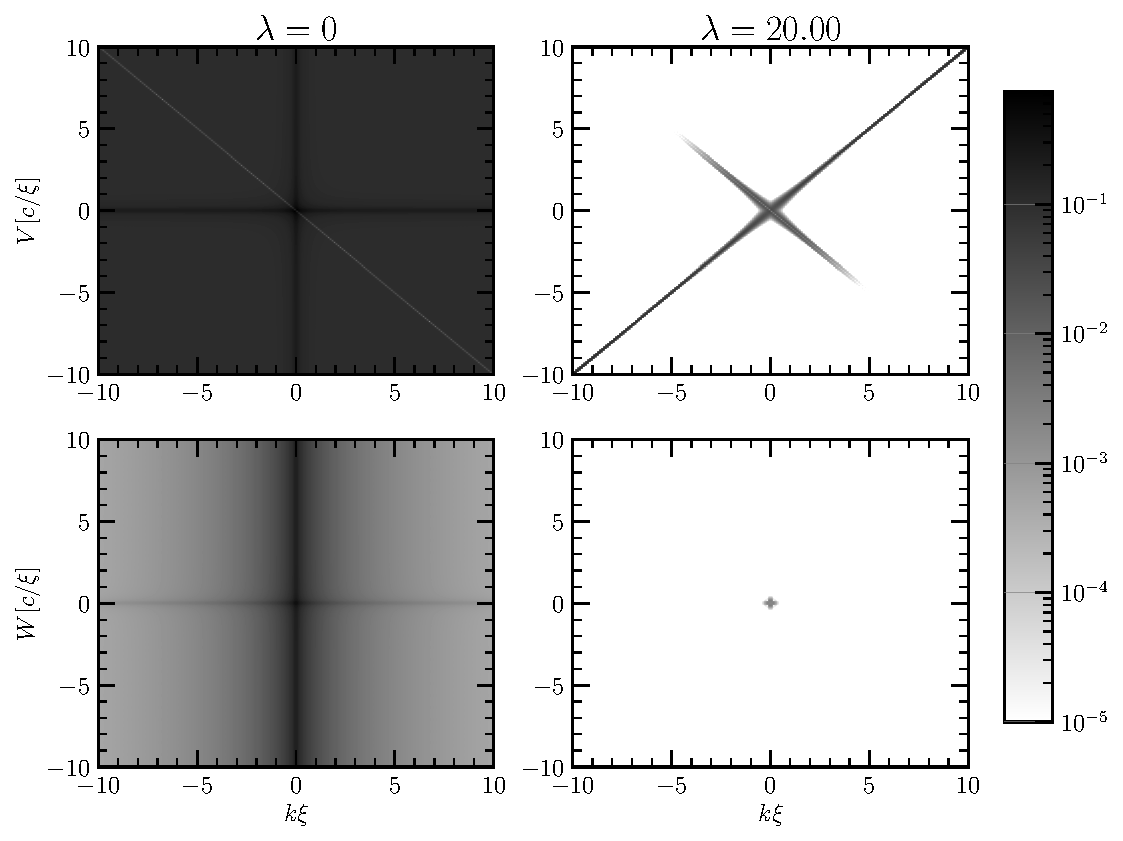
\includegraphics[width=\textwidth]{figures/plots/PDF/FlowIllustration.pdf}
    \caption{Visualization of how the flow progresses for $\eta=10$ by shading larger absolute values for $V_{k,k^\prime},W_{k,k^\prime}$ darker. We see that good suppression occurs for all $W_{k,k^\prime}$, with slower convergence for smaller $|k|,|k^\prime|$.  Meanwhile, the matrix elements near the diagonal $V_{k,k}$ decay significantly slower than most off-diagonal elements. Also, matrix elements $V_{k,-k}$ converge, but to a value different from zero. Note that the values of $V$ near the main diagonal would  become even smaller if the flow were to progress further.}
    \label{FlowIllustration}
\end{figure}
As seen in Figure \ref{FlowIllustration}, the flow equations achieve the desired diagonalization except for terms $V_{k,-k}$. This is because $\omega_k=\omega_{-k}\forall k$ implies that the first order contribution in $\partial_\lambda V_{k,-k} =...$ vanish. This is not a problem for the diagonal terms $V_{k,k}$ because those have been "manually" set to zero by moving them in the diagonal part of the Hamiltonian. 
\subsection{Using a Bogoliubov Transformation}
\section{Comparison of the two Approaches}